\documentclass[runningheads,a4paper]{llncs}
\usepackage{graphicx}
\usepackage{listings}
\usepackage{amssymb}
\usepackage{amsmath}
\usepackage{diagbox}
\usepackage{subcaption}
\usepackage{hyperref}
\usepackage{array}
    \newcolumntype{P}[1]{>{\centering\arraybackslash}p{#1}}
\usepackage{array}
\usepackage{booktabs}
\usepackage{lipsum}
\usepackage[super]{natbib}
\usepackage{setspace}
\usepackage{tabularx}
\usepackage{float}
\usepackage{xcolor}
%\usepackage{fixltx2e}

%define the conditions environment
\newenvironment{conditions}
  {\par\setlength{\leftskip}{1cm}\vspace{\abovedisplayskip}\noindent
   \tabularx{0.9\columnwidth}{>{$}l<{$} @{${}\ =\ {}$} >{\raggedright\arraybackslash}X}}
  {\endtabularx\par\setlength{\leftskip}{1cm}\vspace{\belowdisplayskip}}

%footnote numbering style - roman == roman numerals
\renewcommand{\thefootnote}{\roman{footnote}}

\usepackage[textwidth=14cm, centering]{geometry}
%
%no hyphenation
\usepackage[none]{hyphenat}
\sloppy
%
%
%reference item separation
\newlength{\bibitemsep}\setlength{\bibitemsep}{.35\baselineskip plus .05\baselineskip minus .05\baselineskip}
\newlength{\bibparskip}\setlength{\bibparskip}{0pt}
\let\oldthebibliography\thebibliography
\renewcommand\thebibliography[1]{%
  \oldthebibliography{#1}%
  \setlength{\parskip}{\bibitemsep}%
  \setlength{\itemsep}{\bibparskip}%
}
%
%bibliography column separation width
\setlength{\columnsep}{5mm}
%
%indentation of the first paragraph
\usepackage{indentfirst}
%
%
\usepackage[all]{nowidow} % Tries to remove widows
\usepackage[protrusion=true,expansion=true]{microtype} % Improves typography, load after fontpackage is selected
%
%TC:macro \cite [option:1,1]
%TC:macro \citep [option:1,1]
%TC:macro \citealt [option:1,1]
%
%%%%%%%%%%%%%%%%%%
%%%%%%%%%%%%%%%%%%
%%%%%%%%%%%%%%%%%%
%%%%%%%%%%%%%%%%%%
%%%%%%%%%%%%%%%%%%
%%%%%%%%%%%%%%%%%%
%%%%%%%%%%%%%%%%%%
%%%%%%%%%%%%%%%%%%
%%%%%%%%%%%%%%%%%%
%
\title{\textbf{CELL0014 Report 2}}
\author{\large{Candidate number: xxx}} %LRMV8
\institute{\large{University College London}}
%
\authorrunning{\textbf{xxx | 06/2021 | Word count: xxx}}
%
\begin{document}
%
\maketitle% typeset the header of the contribution

\bigskip
\bigskip
\onehalfspacing
%
\section*{Introduction}
Traditionally, in biology, we focus on the study of naturally occurring systems - attempting to focus on ever-smaller biological mechanisms; trying to decode and understand the tangled web of intertwined processes that living organisms are. Yet, an alternative and a rapidly growing field -- synthetic biology -- has a radically different approach --- using man-designed biological systems which do not only present with an unimaginable number of potential applications for the future (much like the rise of 3D-printing is revolutionising the manufacturing industry), but also offer precious insight into what is required to construct robust, reliable, and predictable biological circuits and genetic networks. Nevertheless, designing \textit{de novo} biological systems is not a straightforward feat, requiring a combination of engineering, mathematics, and both \textit{in silico} and \textit{in vivo} biology.

The Goodwin Oscillator, first theoretically described by Brian Goodwin in the 1960s, is regarded as the first and most simple of the \textit{de novo} biological systems and has since been studied and implemented many times\cite{Gonze2013a, Purcell2010a}. It comprises of a single self-repressing gene, which under the correct set of conditions results in oscillatory rises and falls in the concentration of the genes' product. 

Extending the Goodwin Oscillator are repressilators --- cyclical sets of one or more genes each of which is inhibiting its successor in the set ($1 \dashv 2 \dashv\ ...\ \dashv n \dashv 1$)\cite{Muller2006, Purcell2010a}. The term \textit{Repressilator} was coined by Elowitz and Leibier (2000)\cite{Elowitz2000d} in their influential work describing the first \textit{de novo} oscillatory mechanism \textit{in vivo}. It uses a set of three regulatory genes --- \textit{lacI} from \textit{Escherichia coli} (repressed by cI), \textit{tetR} from the Tn10 transposon (repressed by LacI), and \textit{cI} from the Bacteriophage $\lambda$ (repressed by TetR; see Fig. \ref{fig:fig1})\cite{Elowitz2000d}. In this report, I attempt to revisit the work of Elowitz and Leibier and verify their claims utilising both deterministic and stochastic modelling. First, however, it is paramount to understand the original design of the Repressilator.

\begin{figure}[H]
    \singlespacing
    \centering
    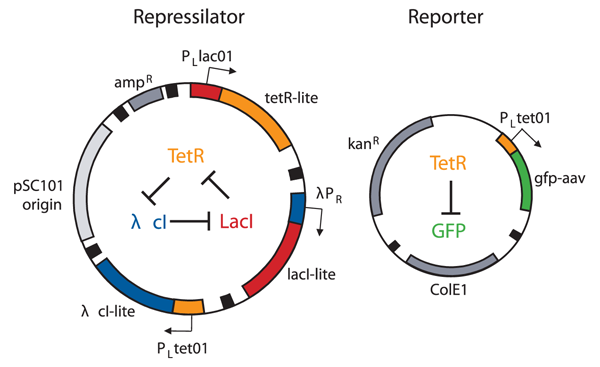
\includegraphics[width=0.95\textwidth]{fig/Repressilator_plasmid.png}
    \caption{\textbf{Repressilator Design.} The Repressilator is composed of three regulatory genes,\linebreak \textit{lacI}, \textit{cI}, and \textit{tetR}, under the control of the P\textsubscript{R} promoter with the cI operator, the P\textsubscript{L} promoter with the TetR operator, and the P\textsubscript{L} promoter with the LacI operator, respectively. The genes are terminated with proteolysis targeting tags (as denoted by the "\textit{lite}" suffix). In addition\linebreak to the Repressilator, the system also includes the Reporter carrying the intermediate-stability GFP (\textit{gfp-avv}) under the control of the P\textsubscript{L}tetO1 promoter allowing to monitor the system state with fluorescent microscopy \textit{in vivo}. The plasmids are equipped with the low-copy pSC101 and the high-copy ColE1 \textit{E. coli} replication origins, and ampicillin and kanamycin resistance genes (allowing to select for cell containing only both plasmids), respectively. T1 terminators from\linebreak the \textit{E. coli rrnB} operon used to isolate the individual open reading frames are shown as black boxes. Gene network diagrams are displayed to illustrate the oscillatory negative-feedback loop circuit. Adapted from Elowitz \& Leibier (2000)\cite{Elowitz2000d}.}
    \label{fig:fig1}
\end{figure}

\subsection*{The Repressilator}
\subsubsection*{Mathematical design:}
Due to the contemporary limited understanding of biochemistry, the team set out to first create a simplistic ordinary differential equation (ODE) model of the biological circuit capturing only the key processes rather than modeling the precise system behaviour. The Repressilator comprises six coupled differential equations:

\vspace{\abovedisplayskip}
\begin{equation*}
    \displaystyle
    \begin{aligned}
        \frac{dm_{i}}{dt}\ =\ -m_{i}+\frac{\alpha}{1+{p_{j}}^{n}}+\alpha_{0} \\[0.5cm]
        \frac{dp_{i}}{dt}\ =\ -\beta(p_{i}-m_{i})
    \end{aligned}
    \hspace{1.2cm}
    \Bigg(\ 
        \begin{aligned}
            i = \textrm{\textit{lacI}, \textit{tetR}, \textit{cI}}    \\
            j = \textrm{\textit{cI}, \textit{lacI}, \textit{tetR}}
        \end{aligned}\ 
    \Bigg)_\textrm{\large{,}}
\end{equation*}

\pagebreak
\noindent where:

\begin{conditions}
    m_{i}               &   mRNA concentration  \\
    p_{i,j}             &   protein concentration   \\
    \alpha_{0}          &   promoter "\textit{leakiness}" (number of mRNA molecules transcribed from the promoter under saturating levels of repressor)  \\
    \alpha+\alpha_{0}   &   number of mRNA molecules transcribed from the promoter produced in the absence of repressor    \\
    \beta               &   ratio of protein decay rate to mRNA decay rate    \\
    n                   &   Hill coefficient (describing binding cooperativity);
\end{conditions}

\noindent all parameters are identical for all three genes, except for their DNA-binding functions; time is rescaled in units of mRNA lifetime; protein concentrations are written in units of K\textsubscript{M} (number of repressor molecules required to reduce the rate of transcription by half); and mRNA concentrations are rescaled by their translation efficiency (average number of proteins produced per mRNA molecule)\cite{Elowitz2000d}. 

After exploring the parameter space (some of which I will engage in below), the authors describe a set of biologically sensible parameters:

\begin{conditions}
    \alpha_{0}                                  &   $5\times 10^{-4}\ [s^{-1}]$  \\
    \alpha+\alpha_{0}                           &   $0.5\ [s^{-1}]$    \\
    \textrm{average translational efficiency}   &   $20\ [\textrm{proteins per transcript}]$  \\
    n                                           &   $2$   \\
    \textrm{protein}\ t_{1/2}                   &   $10\ [\textrm{min}]$    \\
    \textrm{mRNA}\ t_{1/2}                      &   $2\ [\textrm{min}]$, \\
\end{conditions}

\noindent which result in oscillatory rises and falls of the mRNA and protein concentrations\linebreak (see Fig. \ref{fig:fig2})\cite{Elowitz2000d}.

\begin{figure}
    \singlespacing
    \centering
    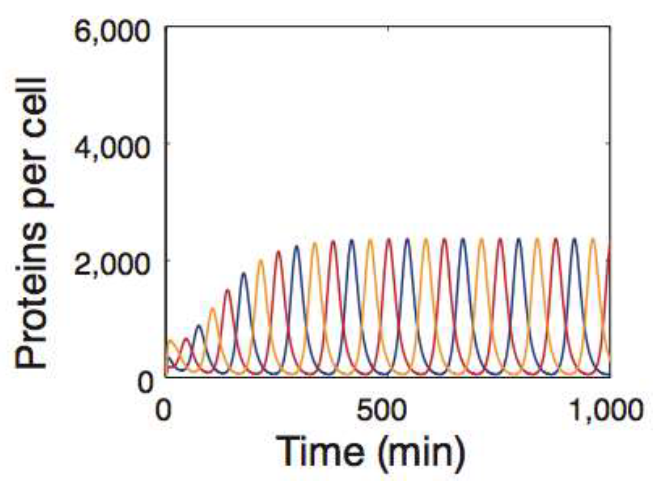
\includegraphics[width=0.45\textwidth]{fig/original_oscilations.png}
    \caption{\textbf{Repressilator protein concentration oscillations.} Color coding as per Fig. \ref{fig:fig1}. Adapted from Elowitz \& Leibier (2000)\cite{Elowitz2000d}.}
    \label{fig:fig2}
\end{figure}

Mathematically, the oscillations are associated with a limit cycle and arise via a super-critical Hopf bifurcation for sufficiently high $n$ under the model proposed above\cite{Purcell2010a, Muller2006, Elowitz2000d}. The Hill function, in the context of transcriptional repression, represents the formation of repressor protein complexes or cooperative binding of repressor to the promoter\cite{Gonze2013a}. This sigmoidal function describes the steepness of the repressional response (as discussed below). In other words, sufficiently boolean repression is required for the Repressilator to produce oscillatory behaviour\cite{Purcell2010a}. Additionally, it is also required for a time delay to exist in the negative feedback loop for repressilators to produce oscillations\cite{Purcell2010a,Gonze2020}.

Generally, repressilators were found to favour strong promoters with low leakiness, high translational efficiency, sufficiently nonlinear repression, the presence of a time delay in the system, and similar protein and mRNA decay rates. Additionally, models (including this document) usually assume all genes and their associated parameters to be identical\cite{Purcell2010a}, however, that can be biologically unpractical/unfeasible, and it has been shown that even unsymmetrical repressilator systems can produce oscillations\cite{Strelkowa2010}. Lastly, repressilator systems seem to prefer odd-numbered sets of genes, nevertheless, there is some evidence that oscillating solutions exist even for $6+$ even-numbered sets and it might thus be only two- (which can form stable on/off switches) and four-membered sets of genes that are unable to produce oscillating behaviour\cite{Purcell2010a,Strelkowa2010}.

\subsubsection*{Biological design:} 
After exploring the circuit design \textit{in silico}, the team set out to create the Repressilator \textit{in vivo}. They resulted to utilising the P\textsubscript{L} promoter  combined with LacI and TetR operator sequences to control the expression of \textit{tetR} and \textit{cI}, respectively, and the P\textsubscript{R} promoter containing the cI operator to control the expression of \textit{lacI} (both promoters originating from the Bacteriophage $\lambda$; see Fig. \ref{fig:fig1}) for their strong expression and tight repression\cite{Elowitz2000d}. 

Such constructed reading frames were cloned into a low-copy plasmid and transformed into the \textit{E. coli} MC4100 $\Delta$(argF-lac)U169 strain with the Lac operon disabled to reduce interference between the Repressilator and the \textit{E. coli} metabolism\cite{Elowitz2000d}. Additionally, Elowitz and Leibier also transformed their bacteria with a high-copy plasmid "\textit{Reporter}", which was carrying the intermediate-stability green fluorescent protein variant (\textit{gfp-aav}; with $t_{1/2} \approxeq 30-40$ min)\cite{Andersen1998} under the control of the P\textsubscript{L}tetO1 to allow for a fluorescent readout of the circuit state (see Fig. \ref{fig:fig1})\cite{Elowitz2000d}. To reduce the relatively high protein half-life to be more comparable with the half-life of mRNA, as required by the model, the team also inserted ssrA tags (making it a target recognised by \textit{E. coli} proteases) at the 3' ends of the genes \cite{Elowitz2000d}.

As mentioned before, at the time of publication, many of the critical parameters were poorly known and thus it was not clear whether the system will indeed oscillate when tested \textit{in vivo}. Conveniently, to the pleasure of the team, at least $40\ \%$ of the cells exhibited oscillatory blinking of green light radiating from the GFP regulated by the Repressilator with peak-to-peak frequency of $160 \pm 40$ min (mean $\pm$ s.d.; notably, roughly threefold longer than the average cell-division time in the experiment)\cite{Elowitz2000d}. 

Additionally, the team also observed significant noise in the oscillatory behaviour, both, in-between mother-daughter and daughter-daughter cells with cells skipping and delaying oscillations\cite{Elowitz2000d}. Even though it was later shown that this erraticity was to a certain extent caused by the limited imaging technology available at the time\cite{Potvin-Trottier2016a}, this chaotic behaviour can to a large degree be accounted to the inherent randomness and stochasticity of living organisms and the universe. For that reason, the researchers also explored a stochastic simulation of the Repressilator using the Gillespie algorithm (some of which I do myself later in this report) showing that the modelled system behaved not dissimilarly to the \textit{in vivo} observations\cite{Elowitz2000d}.

\subsubsection*{Future improvements:}
It is worth mentioning that since its publication in 2000, the design by Elowitz and Leibier has been subject to numerous investigations which yielded much insight into the dynamics of the system\cite{Purcell2010a}. Most notably, recent study by Potvin-Trottier \textit{et al.} (2016)\cite{Potvin-Trottier2016a}\linebreak where the team set out to minimise noise in the original Repressilator - with great success. Instead of adding extra redundant or regulatory mechanisms to the Repressilator, the team focused on achieving the best performace with the most minimalistic design possible.

Firstly, they showed that poor segregation of the high-copy Reporter caused significant fluctuations in the mother-daughter levels of GFP and just moving P\textsubscript{L}tetO1 \textit{gfp-aav} onto the more stable low-copy Repressilator alone lowered the fluorescence amplitude standard deviation from the original $78\ \%$ to $36\ \%$\cite{Potvin-Trottier2016a}. 

Secondly, the team described another significant source of noise - the \textit{E. coli} protein degradation machinery, which can be over-saturated when both the intermediate-stability GFP and the reporter proteins are being targeted for degradation via the ssrA-tags\cite{Potvin-Trottier2016a}. And while it extended the period from 2.4 to 5.7 generations, removing the ssrA-tags from the reporter genes (or lowering the number of gene copies), it strongly improved the accuracy of oscillations allowing the experiment to run for 5.5 cell-cycles before accumulating 0.5 period of drift\cite{Potvin-Trottier2016a}.

Lastly, Potvin-Trottier \textit{et al.} also showed that, the strength of TetR's repression is so high, that even an extremely low number of it's molecules can terminate promoter transcription, which subjects it's regulation under a large amount of stochastic noise. Increasing TetR's repression threshold, by adding additional "soaker" binding sites, greatly reduced the noise all steps in the circuit\cite{Potvin-Trottier2016a}. Such repressor titration could be a very useful and important tool for tuning synthetic networks to specific behaviour or for designing very precise switches.

Repressilator modified in this fashion was able to reliably display 14-generation periods (with the above-described accuracy) under a wide range of conditions, showing that the ability to carefully tweak biochemical parameters and a deep understanding of the stochastic nature of the relevant biochemical processes can produce astonishingly precise and predictable fashion even in such primitive circuit\cite{Potvin-Trottier2016a}.

\section*{Analysis}
Alongside discussing the Repressilator's design and relevance, this document also aims to revisit the original work by Elowitz and Leibier\cite{Elowitz2000d} and reconfirm their claims and provide additional insight into the system's behaviour.

Expanding the original ODEs, we arrive at set of equations:

\begin{equation*}
    \begin{aligned}
        \partial^{+}m_{i}({\scriptstyle t,\ t+1})\ =\ k_{m}\frac{K^{n}}{K^{n}+{P_{j}({\scriptstyle t})}^{n}}+{k_{m}}_{0} \\[0.1cm]
        \partial^{+}P_{i}({\scriptstyle t,\ t+1})\ =\ k_{p}*{m_{i}({\scriptstyle t})} \\[0.2cm]
        \partial^{-}m_{i}({\scriptstyle t,\ t+1})\ =\ k_{dm}*{m_{i}({\scriptstyle t})} \\[0.1cm]
        \partial^{-}P_{i}({\scriptstyle t,\ t+1})\ =\ k_{dp}*{P_{i}({\scriptstyle t})} \\[0.3cm]
        \Delta m_{i}({\scriptstyle t,\ t+1})\ =\ \partial^{+}m_{i}({\scriptstyle t,\ t+1})\ -\ \partial^{-}m_{i}({\scriptstyle t,\ t+1}) \\[0.1cm]
        \Delta P_{i}({\scriptstyle t,\ t+1})\ =\ \partial^{+}P_{i}({\scriptstyle t,\ t+1})\ -\ \partial^{-}P_{i}({\scriptstyle t,\ t+1}) \\[0.3cm]
        m_{i}({\scriptstyle t+1})\ =\ m_{i}({\scriptstyle t}) + \Delta m_{i}({\scriptstyle t,\ t+1}) \\[0.1cm]
        P_{i}({\scriptstyle t+1})\ =\ P_{i}({\scriptstyle t}) + \Delta P_{i}({\scriptstyle t,\ t+1})
    \end{aligned}
    \hspace{0.8cm}
    \Bigg(\ 
        \begin{aligned}
            i = \textrm{\textit{lacI}, \textit{tetR}, \textit{cI}}    \\
            j = \textrm{\textit{cI}, \textit{lacI}, \textit{tetR}}
        \end{aligned}\ 
    \Bigg)_\textrm{\large{,}}
\end{equation*}
    
\noindent where\footnote{All parameter values have been converted from the original Repressilator parameters described above (see Supplementary Information for detailed calculations).}:

\begin{conditions}
    t   &   time [min]    \\
    K   &   $40$ (repression K\textsubscript{M}, number of repressor molecules required to reduce expression by $50\ \%$)    \\
    n   &   $2$ (Hill coefficient)  \\
    P_{i,j}({\scriptstyle t})   &   number of protein molecules at time $t$\\
    m_{i}({\scriptstyle t})   &   number of mRNA molecules at time $t$\\
    k_{m}   &   $30\ [\textrm{min}^{-1}]$ (maximum rate of transcription; $\alpha + \alpha_{0}$)    \\
    {k_{m}}_{0}  &   $0.03\ [\textrm{min}^{-1}]$ (promoter ”leakiness; $\alpha_{0}$)  \\
    k_{p}   &   $6.931\ [\textrm{min}^{-1}]$ (translational efficiency) \\    
    k_{dm}   &   $0.3466\ [\textrm{min}^{-1}]$ (rate of mRNA decay)    \\
    k_{dp}   &   $0.06931\ [\textrm{min}^{-1}]$ (rate of protein decay),  \\
\end{conditions}

\noindent assuming saturated transcription and translation, which can be used to model the mRNA and protein levels across time. In the chapters below, I discussed how I used these equations implemented in Python to study the Repressilator system. All code used to conduct this analysis is attached as part of the Supplementary Information.

\clearpage
\subsection*{Task 1}
First, let us consider a simplified scenario with only two genes out of the three regulatory genes -- \textit{lacI} and \textit{tetR}:

\begin{equation*}
    P_{\textrm{lacI}} \dashv P_{\textrm{tetR}}
\end{equation*}

\noindent where we are concerned only with two out of the six ODEs describing the Repressilator ($m_{i}\ \&\ P_{i};\ i\ =\ \textrm{\textit{tetR}},\ j\ =\ \textrm{\textit{lacI}}$). Assuming constant levels of LacI, we can examine the steady-state (once the system has reached it; $t_{\textrm{\tiny MAX}}=1000\ [\textrm{min}]$) concentration of TetR under different parameters --- namely, the Hill coefficient. This will allow us to see how different levels of cooperativity affect the repression kinetics between LacI and TetR under the model described above\footnote{Initial conditions: $m_{\textrm{\textit{tetR}}}({\scriptstyle t=0}) =\ 0$, $P_{\textrm{TetR}}({\scriptstyle t=0}) =\ 5$} (see Fig. \ref{fig:fig3}). 

\begin{figure}
    \singlespacing
    \centering
    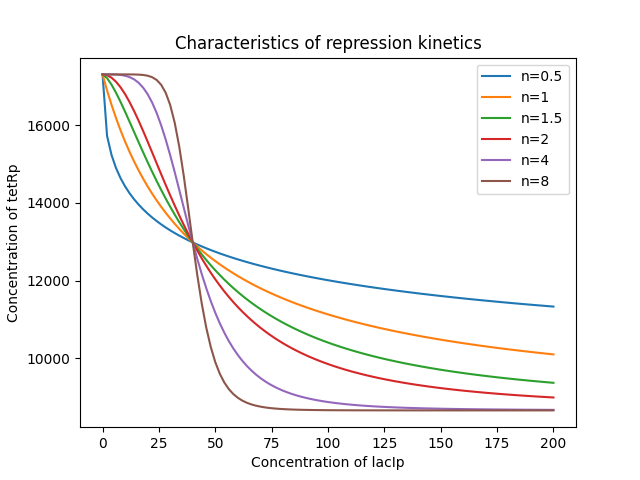
\includegraphics[width=0.75\textwidth]{suplementary_information_and_code/Task1_figure1.png}
    \caption{\textbf{Characteristics of repression kinetics in the isolated system of $P_{\textrm{lacI}} \dashv P_{\textrm{tetR}}$.} With growing $n$ (Hill coefficient), repression of TetR production by LacI becomes more sigmoidal and boolean. Sufficiently high $n$ ($\gtrapprox 1.64$; see Fig. \ref{fig:fig9}) is required to produce a Hopf bifurcation and for the system to oscillate. All curves converge at LacI $= 40$ ($K$; concentration of LacI required to reduce \textit{tetR} expression by $50 \%$).}
    \label{fig:fig3}
\end{figure}

I have tested $n$ ranging from 0.5 (negative cooperativity), 1.0 (no cooperativity), to 8.0 (high positive cooperativity) --- a biologically relevant range (in the context of transcriptional repression, it is almost impossible to reach Hill coefficients over 4\cite{Gonze2013a}). In the simulation we can observe that with the Hill coefficient increasing, the repression curve of $P_{\textrm{lacI}} \dashv P_{\textrm{tetR}}$ grows steeper - decreasing the number of molecules required to switch the gene expression state (while $K$ stays fixed). Biologically, this behaviour could be explained either by repressor protein multimerisation (increasing the affinity of biding to the operator, or by cooperative binding (where repressor protein binding to the operator increases the binding affinity for other repressor molecules\cite{Gonze2013a}.

\subsection*{Task 2}
Now, let us consider the full Repressilator circuit as described above\footnote{Initial conditions (used throughout the analysis, unless stated otherwise): $m_{\textrm{\textit{lacI}}}({\scriptstyle t=0}) =\ 0$, $m_{\textrm{\textit{tetR}}}({\scriptstyle t=0}) =\ 0$, $m_{\textrm{\textit{cI}}}({\scriptstyle t=0}) =\ 0$, $P_{\textrm{LacI}}({\scriptstyle t=0}) =\ 0$, $P_{\textrm{TetR}}({\scriptstyle t=0}) =\ 5$, and $P_{\textrm{cI}}({\scriptstyle t=0}) =\ 0$}. When simulated for $1000\ \textrm{min}$, the system exhibited stable and indefinite (as they are associated with a limit cycle; see below) oscillatory rises and falls in the regulatory-proteins' concentrations consistent with the results reported by Elowitz and Leibier in 2000 (see Fig. \ref{fig:fig2} and Fig. \ref{fig:fig4})\cite{Elowitz2000d}.

\vspace{-3\abovedisplayskip}
\begin{figure}
    \singlespacing
    \centering
    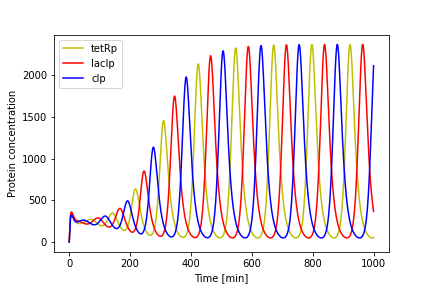
\includegraphics[width=0.70\textwidth]{suplementary_information_and_code/Task2_figure1.png}
    \caption{\textbf{Repressilator ODE simulation results.} It is clear, that the Repressilator system as described as above does indeed produce an oscillatory behaviour of the regulatory protein concentrations \textit{in silico}. After a transient period, after the system reaches the limit cycle, the peak amplitude $\approxeq 2500\ \textrm{molecules}$, and the peak-to-peak period $\approxeq 125\ \textrm{min}$. Colour coding as per Fig. \ref{fig:fig1}.}  
    \label{fig:fig4}
\end{figure}

In addition to the limit cycle oscillations, the system can also enter a steady state as per the assumption that all gene parameters are identical. This steady state arises when the initial conditions for all three genes are also identical ($P_{\textrm{LacI}}({\scriptstyle t=0}) = P_{\textrm{TetR}}({\scriptstyle t=0}) = P_{\textrm{cI}}({\scriptstyle t=0})\ \wedge\ m_{\textrm{\textit{lacI}}}({\scriptstyle t=0}) = m_{\textrm{\textit{tetR}}}({\scriptstyle t=0}) = m_{\textrm{\textit{cI}}}({\scriptstyle t=0})$) as shown in Fig. \ref{fig:fig5}. However, should even only a minuscule difference exist between the three sets of initial conditions (for each gene) exist, the system will eventually reach the limit cycle and produce oscillations as shown in Fig. \ref{fig:fig6}.

\begin{figure}
    \singlespacing
    \centering
    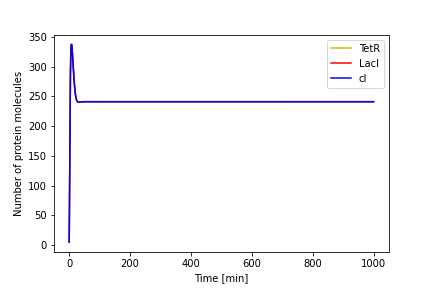
\includegraphics[width=0.70\textwidth]{suplementary_information_and_code/Task2_figure2.png}
    \caption{\textbf{Repressilator ODE simulation of steady-state.} Instead of producing oscillations, the system enters a steady state ($P_{\textrm{\tiny ALL}} \approxeq 240\ [\textrm{molecules}]$) when the initial conditions for all three genes are identical. Note that only the curve representing the cI concentration is visible, as all plotted concentrations are identical and overlap. Initial conditions: $m_{\textrm{\textit{lacI}}}({\scriptstyle t=0}) =\ 0$, $m_{\textrm{\textit{tetR}}}({\scriptstyle t=0}) =\ 0$, $m_{\textrm{\textit{cI}}}({\scriptstyle t=0}) =\ 0$, $P_{\textrm{LacI}}({\scriptstyle t=0}) =\ 5$, $P_{\textrm{TetR}}({\scriptstyle t=0}) =\ 5$, and $P_{\textrm{cI}}({\scriptstyle t=0}) =\ 5$. Colour coding as per Fig. \ref{fig:fig1}.}  
    \label{fig:fig5}
\end{figure}

\begin{figure}
    \centering
    \singlespacing
    \noindent\makebox[\textwidth]{
        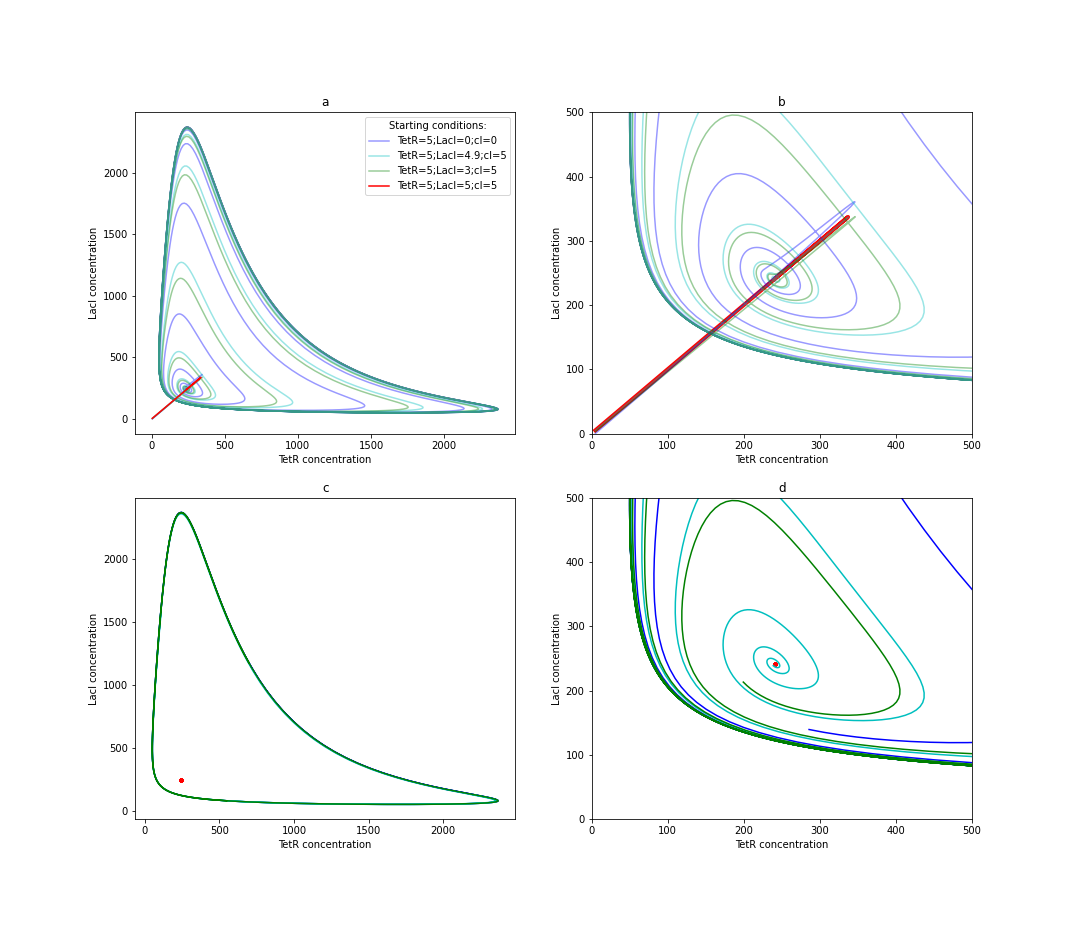
\includegraphics[width=18cm, trim={2cm 2cm 2cm 3.5cm},clip]{suplementary_information_and_code/Task2_figure3.png}}
    \caption{\textbf{Repressilator ODE Phase plot.} This plot is showing the relation of TetR and LacI concentrations, nevertheless, the system comprises of 3 genes. To be able to completely understand the system behaviour, a 3D representation is required (See Supplementary Information). \textbf{(\textit{a})} Repressilator simulations ($t_{\textrm{\tiny MAX}}=1000\ \textrm{min} $) with different starting protein concentrations are shown (all mRNA concentrations $= 0$). Regardless the starting conditions (unless they are on the limit cycle), the system will promptly colapse close near the steady state and, unless started with all concentrations identical (in which case the system will enter the steady state), the system will start approaching the limit cycle. The steady state simulation is shown in red; its linear trajectory represents the system behaviour in Fig. \ref{fig:fig5} where the protein concentrations reach the steady state after a short period of transient rise and fall, with all concentrations being identical. \textbf{(\textit{b})} Showing simulations as in \textit{\textbf{a}}, but cropped to better show the steady state a identical simulation approaches to the limit cycle. \textbf{(\textit{c})} Showing simulations as in \textit{\textbf{a}} with the initial transient behaviour (first $800\ \textrm{min}$ of simulation) removed - showing that all simulations except for the steady state (shown in red) are associated with the limit cycle. \textbf{(\textit{d})} Showing simulations as in \textit{\textbf{a}} with the initial $200\ \textrm{min}$ (once the steady state simulation arrived at the steady state) removed to show that while, the the initial conditions might be almost identical and the system will come very close to the steady state, it will always eventually reach the limit cycle (the closer the initial conditions to being identical, the longer it will take for the system to reach the limit cycle; see Supplementary Information).}
    \label{fig:fig6}
\end{figure}

\clearpage
\subsection*{Task 3}
In previous Tasks, we have examined how the Hill coefficient affects the repression profile, and how the Repressilator produces oscillations. Here, I will demonstrate how the Hill affects the system behaviour. 

When we simulate the Repressilator with all parameters as outlined above, except for setting the Hill coefficient to a sub-critical level ($\lessapprox 1.64$; see Fig.\ref{fig:fig9}) for the Hopf bifurcation to arise ($n = 1.3$), the system will not produce oscillations, but will rather settle at a steady state ($P_{\textrm{\tiny ALL}} \approxeq 420\ [\textrm{molecules}]$; see Fig. \ref{fig:fig7}). Extending this approach and simulating over a range of $n$ (see Fig. \ref{fig:fig8}), shows what a drastic effect the Hill coefficient has on the behaviour of the Repressilator. When $n$ becomes super-critical, as $n$ increases, so does the oscillation peak amplitude (see Fig. \ref{fig:fig9}), while the peak-to-peak period is unchanged (data not shown).

\vspace{-3\abovedisplayskip}
\begin{figure}
    \singlespacing
    \centering
    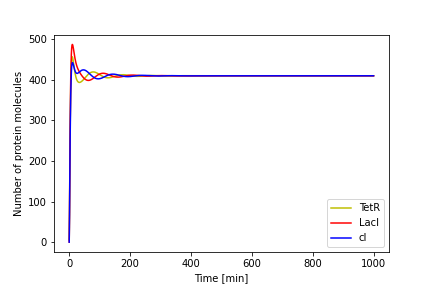
\includegraphics[width=0.75\textwidth]{suplementary_information_and_code/Task3_figure1.png}
    \caption{\textbf{Repressilator ODE simulation with sub-critical $n$.}}
    \label{fig:fig7}
\end{figure}

\begin{figure}
    \singlespacing
    \centering
    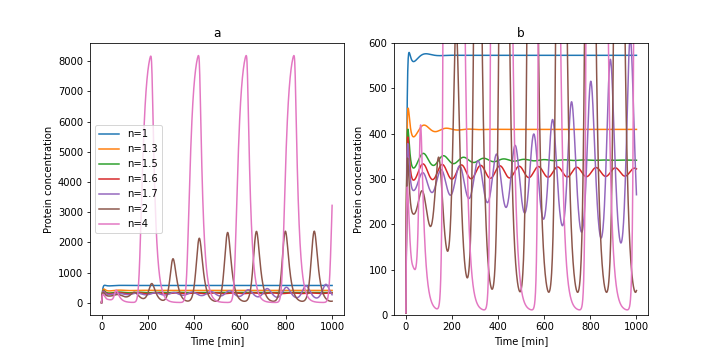
\includegraphics[width=\textwidth]{suplementary_information_and_code/Task3_figure2.png}
    \caption{\textbf{Repressilator ODE simulation over range of $n$.} \textbf{(\textit{a})} With increasing $n$, the system behaviour changes. When $n$ rises above the super-critical level ($\gtrapprox 1.64$; see Fig. \ref{fig:fig9}) and a Hopf bifurcation arises in the system, oscillations emerge. The repressilator was simulated over a biologically relevant range of Hill coefficients, as stipulated above. \textbf{(\textit{b})} Showing simulations as in \textbf{\textit{a}}, but cropped to better illustrate the fine transition from sub- to super-critical $n$.}
    \label{fig:fig8}
\end{figure}

\begin{figure}
    \singlespacing
    \centering
    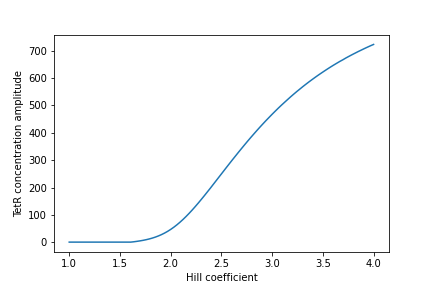
\includegraphics[width=0.75\textwidth]{suplementary_information_and_code/Task3_figure3.png}
    \caption{\textbf{Protein peak amplitude in relation to changing $n$.} When $n$ crosses the super-critical level ($\gtrapprox 1.64$), oscillations occur in the system and with increasing $n$, the peak concentration amplitude rises as well (data only for TetR shown, but the relationship of $n$ to peak amplitude is identical for all three Repressilator genes).}
    \label{fig:fig9}
\end{figure}

Additionally, in this section, I will also examine how additional system parameters --- translational efficiency ($k_{p}$; see Fig. \ref{fig:fig10}) and promoter leakiness (${k_{m}}_{0}$; $\alpha_{0}$; see Fig. \ref{fig:fig11}). It can be seen the relationship between the rate of translation and the peak concentration amplitude resembles a $\Gamma$ distribution, with its peak $\approxeq 12$. This can be interpreted as the fact that, too low of an efficiency is not able to produce enough protein before the next oscillation, however, too high of a translational efficiency and the genes expression will be silenced a sufficient amount of mRNA can be produced. In the context of promoter leakiness, the protein amplitude decreases drastically with growing leakiness, and as ${k_{m}}_{0}$ approaches $0.068$, the system seizes to oscillate. This observation can likely be explained by the fact that the background expression of the Repressilator is so high, that the promoters are constantly under saturating levels of repressors.

\begin{figure}
    \singlespacing
    \centering
    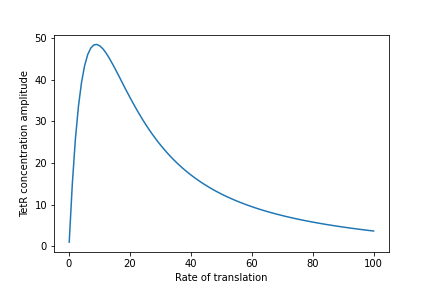
\includegraphics[width=0.75\textwidth]{suplementary_information_and_code/Task3_figure4.png}
    \caption{\textbf{Repressilator ODE simulation over range of $k_{p}$.} Data only for TetR shown, but the relationship of $k_{p}$ to peak amplitude is identical for all three Repressilator genes.}
    \label{fig:fig10}
\end{figure}

\begin{figure}
    \singlespacing
    \centering
    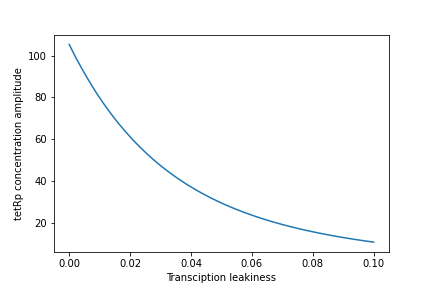
\includegraphics[width=0.75\textwidth]{suplementary_information_and_code/Task3_figure5.png}
    \caption{\textbf{Repressilator ODE simulation over range of ${k_{m}}_{0}$.} Data only for TetR shown, but the relationship of ${k_{m}}_{0}$ to peak amplitude is identical for all three Repressilator genes.}
    \label{fig:fig11}
\end{figure}

\clearpage
\subsection*{Task 4}
After having explored the Repressilator parameter space, let us examine behaviour of the system when we include the expression of GFP as controlled on the Reporter. This requires the addition of two differential equations into our system --- $m_{\textrm{\textit{gfp}}}$ and $P_{\textrm{GFP}}$:

\begin{equation*}
    \begin{aligned}
        \partial^{+}m_{\textrm{\textit{gfp}}}({\scriptstyle t,\ t+1})\ =\ k_{m}\frac{K^{n}}{K^{n}+{P_{\textrm{TetR}}({\scriptstyle t})}^{n}}+{k_{m}}_{0} \\[0.1cm]
        \partial^{+}P_{\textrm{GFP}}({\scriptstyle t,\ t+1})\ =\ k_{p}*{m_{\textrm{\textit{gfp}}}({\scriptstyle t})} \\[0.2cm]
        \partial^{-}m_{\textrm{\textit{gfp}}}({\scriptstyle t,\ t+1})\ =\ k_{dm}*{m_{\textrm{\textit{gfp}}}({\scriptstyle t})} \\[0.1cm]
        \partial^{-}P_{\textrm{GFP}}({\scriptstyle t,\ t+1})\ =\ {k_{dp}}_{\textrm{GFP}}*{P_{\textrm{GFP}}({\scriptstyle t})} \\[0.3cm]
        \Delta m_{\textrm{\textit{gfp}}}({\scriptstyle t,\ t+1})\ =\ \partial^{+}m_{\textrm{\textit{gfp}}}({\scriptstyle t,\ t+1})\ -\ \partial^{-}m_{\textrm{\textit{gfp}}}({\scriptstyle t,\ t+1}) \\[0.1cm]
        \Delta P_{\textrm{GFP}}({\scriptstyle t,\ t+1})\ =\ \partial^{+}P_{\textrm{GFP}}({\scriptstyle t,\ t+1})\ -\ \partial^{-}P_{\textrm{GFP}}({\scriptstyle t,\ t+1}) \\[0.3cm]
        m_{\textrm{\textit{gfp}}}({\scriptstyle t+1})\ =\ m_{\textrm{\textit{gfp}}}({\scriptstyle t}) + \Delta m_{\textrm{\textit{gfp}}}({\scriptstyle t,\ t+1}) \\[0.1cm]
        P_{\textrm{GFP}}({\scriptstyle t+1})\ =\ P_{\textrm{GFP}}({\scriptstyle t}) + \Delta P_{\textrm{GFP}}({\scriptstyle t,\ t+1})\textrm{\large{,}}
    \end{aligned}
\end{equation*}

\noindent where all parameters are identical as outlined above except for GFP $t_{1/2} = 60\ [\textrm{min}]$\linebreak (${k_{dp}}_{\textrm{GFP}} = 0.01155\ [\textrm{min}^{-1}]$) to reflect its lower degradation rate compared to the Repressilator proteins. The simulation (see Fig. \ref{fig:fig12}) shows results comparable with those seen originally by Elowitz and Leibier\cite{Elowitz2000d}.

\vspace{-2.2\abovedisplayskip}
\begin{figure}[H]
    \singlespacing
    \centering
    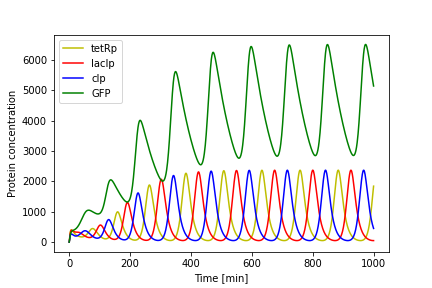
\includegraphics[width=0.75\textwidth,trim={0 0.1cm 0 1.2cm},clip]{suplementary_information_and_code/Task4_figure1.png}
    \caption{\textbf{Repressilator ODE simulation with GFP.} The system simulation produces oscillations in protein concentration for both the Repressilator genes and the \textit{gfp}. Notably, GFP minimal amplitude corresponds to the of cI as predicted by the model (both being controlled by a TetR operator). Additionally, it can be seen that the GFP concentration never returns to 0 as it does with the rest of the genes. This is due GFP's comparably\linebreak longer $t_{1/2}$. Colour coding as per Fig. \ref{fig:fig1}.}
    \label{fig:fig12}
\end{figure}

\subsection*{Task 5}
Let us consider options for finer control of the Repressilator. In this section, I introduce IPTG induction and control of the protein degradation rate (e.g. via variable levels of proteases) in the system. This could be useful to gain a finer control over the system and for added potential functionality. 

\subsubsection*{IPTG Induction}
IPTG can be used to "\textit{soak}" LacI and thus control the expression levels of \textit{tetR}. To introduce the IPTG induction into the system, we need to modify the ODE describing the production of \textit{tetR} mrNA as follows:

\begin{equation*}
    \partial^{+}m_{\textrm{\textit{tetR}}}({\scriptstyle t,\ t+1})\ =\ k_{m}\frac{K^{n}}{K^{n}+(\textcolor{red}{X}*{P_{\textrm{LacI}}({\scriptstyle t})}^{n})}+{k_{m}}_{0}
\end{equation*}

\noindent where $X$ represents the proportion of available LacI not-bound to IPTG (i.e. IPTG concentration). Simulating this system with different concentrations of IPTG lends us insight into how it affects the Repressilator. With rising levels of IPTG (see Fig. \ref{fig:fig13} and \ref{fig:fig14}), we can see both amplitude and frequency of TetR oscillations plummet and eventually reach a steady state ($P_{\textrm{TetR}} \approxeq 9000\ [\textrm{molecules}]$) as we remove any affect of LacI onto the \textit{tetR} promoter with saturating levels of IPTG.

\begin{figure}
    \singlespacing
    \centering
    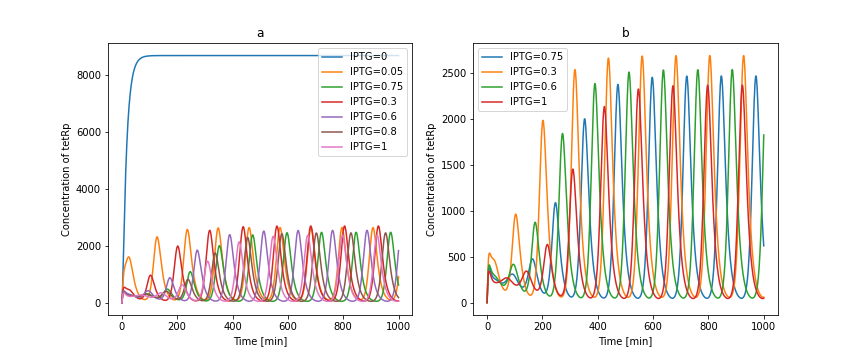
\includegraphics[width=1\textwidth,trim={1.5cm 0 1.5cm 0},clip]{suplementary_information_and_code/Task5_figure1.png}
    \caption{\textbf{Repressilator ODE simulation over a range of IPTG concentrations.} \textbf{(\textit{a})} Overlay of Repressilator simulations at different IPTG concentrations. \textbf{(\textit{b})} Showing a selection of simulations as in \textbf{\textit{a}} to better show the effect of lower IPTG concentrations on the Repressilator.}
    \label{fig:fig13}
\end{figure}

\begin{figure}[h]
    \singlespacing
    \centering
    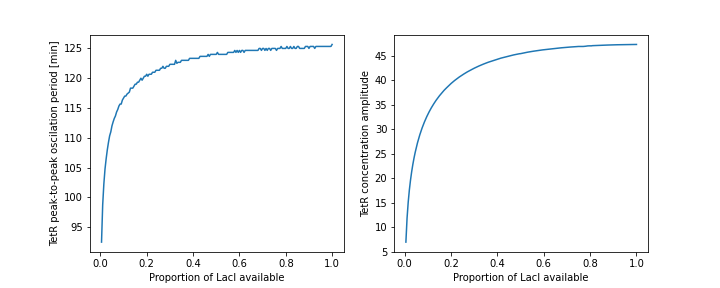
\includegraphics[width=1\textwidth,trim={1.5cm 0 1.5cm 0},clip]{suplementary_information_and_code/Task5_figure2.png}
    \caption{\textbf{Repressilator protein oscillatory period and amplitude over a range of IPTG concentrations.}}
    \label{fig:fig14}
\end{figure}

\subsubsection*{Protein Degradation Rate}
To introduce the protein degradation rate modulation into the system, we need to modify the ODE describing protein degradation as follows:

\begin{equation*}
    \partial^{-}P_{i}({\scriptstyle t,\ t+1})\ =\ \textcolor{red}{Y}*k_{dp}*{P_{i}({\scriptstyle t})}
    \hspace{0.8cm}
    \big(i\ =\ \textrm{\textit{lacI}, \textit{tetR}, \textit{cI}}\big)
\end{equation*}

\noindent where $Y$ represents the repression modulation factor ($Y = 0.167 \rightarrow {t_{1/2}}_{\textrm{P}} = 60\ [\textrm{min}]$, $Y = 5 \rightarrow {t_{1/2}}_{\textrm{P}} = 2\ [\textrm{min}]$). From the simulation results (see Fig. \ref{fig:fig15} and \ref{fig:fig16}), we can infer that while protein degradation does not affect the final oscillation period (while it critically affects how much time is it going to take the system until it reaches the limit cycle), it certainly affects the oscillation amplitude --- after a short period of the system reaching its maximum amplitude, the quicker the protein degradation the lower the amplitude, as not enough protein is able to build up before it gene expression is silenced.

\begin{figure}
    \singlespacing
    \centering
    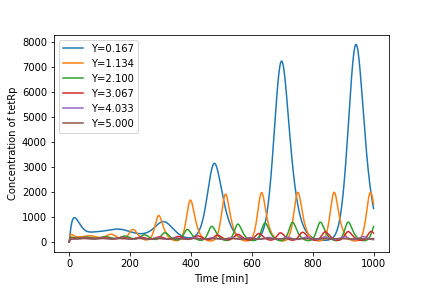
\includegraphics[width=0.75\textwidth]{suplementary_information_and_code/Task5_figure3.png}
    \caption{\textbf{Repressilator ODE simulation over a range of $Y$ levels.}}
    \label{fig:fig15}
\end{figure}

\begin{figure}
    \singlespacing
    \centering
    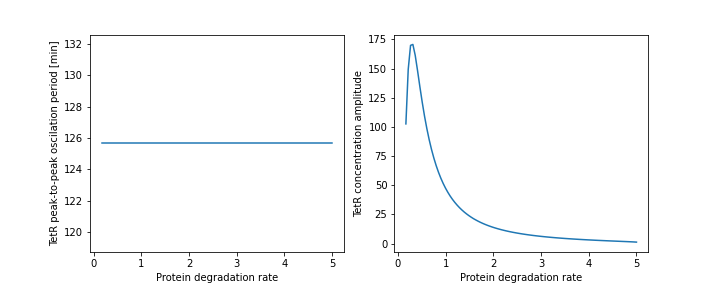
\includegraphics[width=1\textwidth,trim={1.5cm 0 1.5cm 0},clip]{suplementary_information_and_code/Task5_figure4.png}
    \caption{\textbf{Repressilator protein oscillatory period and amplitude over a range of $Y$ levels.}}
    \label{fig:fig16}
\end{figure}

\clearpage
\subsection*{Task 6}
\section*{Discussion}

%
\clearpage
% ---- Bibliography ----
% Find from the left the folder bibliography/ and locate first.bib. you
% can generate your bibtex references using citepthisforme and paste it inside the first.bib file
% to citep a bibliography, use \citep{bisht_hinrichs_skrupsky_venkatakrishnan_2014} (example)
% those are citations embedded to texts
% please check out https://www.latex-tutorial.com/tutorials/bibtex/

%setting bibliography format
\newgeometry{centering, textwidth=15.5cm, textheight=20cm} %normal text height is 20 cm
\singlespacing
\twocolumn
\raggedright
\raggedbottom
\interlinepenalty=10000
%
\small{\bibliography{ref/library.bib}}
\bibliographystyle{ref/vancouver2.bst}
%
\end{document}
